


% \section{Computation and the Computational Mind}
% \section{Language of Thought}
% \section{Grammar}
% - GOFAI
% - Connectionism
% - Hybrid
% - Constructivism
% - Structure
% - Compositional
% \section{Syntax vs Semantics}



\section{Problem Statement}
It has long been hypothesized that our cognition is based on some sort of language of thought (LOT). Recent advances in the field have shown promising results by interpreting this LOT as a type of programming language \cite{rule_child_2020, ellis_dreamcoder_2021, dehaene_symbols_2022}. The language is constructed from the bottom-up using primitives in a domain specific language. However, thus far this has been done purely syntactically. I hypothesize that meaning is not just an emergent phenomenon but a crucial part of concept formation. I therefore propose using graph neural networks and represent program components as nodes, in order to include relational structure. Additionally, nodes can contain supplementary semantic information. This hypothesis will be tested by comparing the resulting model to Ellis et al.'s DreamCoder \cite{ellis_dreamcoder_2021}.

Let's assume the premise that the mind is computational, in one form or another. 
and we are building a world model which can be thought of as probabilistic programs. 

\section{Background}

\subsection{Program Synthesis}

Probabilistic programs, in essence, represent a form of causal reasoning. By representing beliefs as probability distributions and reasoning patterns as programmatic structures, they offer a nuanced way of modeling complex real-world systems. Given the inherently uncertain nature of our environment and the myriad possible interpretations of sensory data, a probabilistic approach is naturally aligned with the cognitive demands of building accurate and adaptable world models.

Program synthesis refers to the automatic generation of programs from a higher-level specification. In the context of cognition, it implies a process where an agent generates a novel programmatic structure to represent or reason about its environment. Understanding this synthesis process becomes crucial for several reasons:

Generativity and Flexibility: Human cognition is not merely reactive. It proactively creates, hypothesizes, and experiments. By studying how programs are synthesized, we might glean insights into the generative aspects of thought.

Abstraction: At the heart of program synthesis is the ability to abstract away from particulars and generate general rules or patterns. This mirrors cognitive abilities like generalization and analogy-making.

Efficiency: Just as efficient algorithms are prized in computing, efficient cognitive strategies are essential for survival. Program synthesis might hold the key to understanding how humans prune vast possibility spaces to arrive at functional solutions quickly.

Moreover, the impressive capabilities of large language models (LLMs) is undeniable, yet they fail at various "simple" tasks, where approaches of formal languages shine. 




Problem Statement: Navigating the Vast Program Search Space Within Context-Free Grammars

1. Background and Introduction

The field of programming has always been underpinned by the intricacies of formal grammars. Context-Free Grammars (CFGs), a subset of formal grammar, are essential in defining the syntactical structures of many programming languages. However, given the generative nature of CFGs, the potential program space defined by even a modestly complex grammar can be immensely vast. Searching for a specific program within this space, or ensuring that a particular space is sufficiently explored, poses significant computational challenges.

2. Problem Definition

2.1 CFG and Program Space

Let \( G = (N, \Sigma, P, S) \) be a Context-Free Grammar, where:
\begin{itemize}
    \item \( N \) is a finite set of non-terminal symbols.
    \item \( \Sigma \) is a finite set of terminal symbols with \newline \( N \cap \Sigma = \emptyset \)
    \item \( P \) is a finite set of production rules, where each rule is of the form \( N \rightarrow (N \cup \Sigma)^* \)
    \item \( S \) is the start symbol, with \( S \in N \)
\end{itemize}

Given such a CFG, the derived program space \( \Pi(G) \) is the set of all possible strings (or sequences of symbols) derivable from \( S \).

2.2 Problem Statement

Given a Context-Free Grammar \( G \) and a defined objective function \( f \) that maps any program \( p \in \Pi(G) \) to a real value representing its desirability or fitness:

Find \( p^* \) such that:
\[ p^* = \arg\max_{p \in \Pi(G)} f(p) \]

In other words, the problem is to locate a program \( p^* \) within the vast program space \( \Pi(G) \) defined by \( G \) that maximizes (or, alternatively, minimizes) the objective function \( f \).

3. Challenges and Complications

3.1 Size of the Search Space

The generative capacity of CFGs means that even grammars of moderate complexity can define immensely vast program spaces. The sheer size of these spaces poses computational and search challenges.

3.2 Non-Linearity and Discontinuities

The mapping between programs and their fitness as defined by \( f \) might be non-linear with multiple local maxima, making search strategies based on gradient ascent or other linear heuristics suboptimal.

3.3 Generalization vs Specialization

While CFGs provide a generalized representation of possible programs, the objective function might lead to highly specialized solutions. Balancing between the two is non-trivial.

3.4 Syntactic vs Semantic Validity

A CFG ensures syntactic validity but does not guarantee semantic correctness. Ensuring that a program derived from a CFG is semantically meaningful or error-free in a given context is an additional layer of complexity.




4. Techniques in Program Synthesis

Several techniques have emerged as pivotal in the domain of program synthesis:

Deductive Synthesis: Rooted in formal logic, this method transforms specifications into programs. The use of logic mirrors certain cognitive tasks, especially those demanding strict reasoning.

Stochastic Search: By randomly exploring the space of possible programs, these methods mirror heuristic-based cognitive processes. Genetic algorithms, for instance, mimic evolutionary processes to evolve optimal or near-optimal solutions.

Neural Program Synthesis: Neural networks, especially recurrent ones, have shown promise in generating programmatic structures. The parallels between neural networks and neural structures in the brain offer tantalizing possibilities for cognitive science.

Example-Based Synthesis: Drawing inspiration from how humans often learn—from examples—these methods generate programs by generalizing from provided instances. This mirrors pedagogical processes and experiential learning.



\section{DreamCoder}
One of the most fascinating undertakings of Artificial Intelligence (AI) is its objective to reveal and learn from the mechanisms of human cognition.

The idea that the thoughts are constructed by some kind of Language of Thought (LOT), in order to understand and represent our reality has a long history. 
Gottfried Leibniz imagined a \textit{Characteristica Universalis}, a formal language capable of expressing metaphysical concepts \cite{sep-leibniz-logic-influence}.
Jerry Fodor, among many other scholars, developed this hypothesis, and proposed that thoughts are composed according to some form of internal grammar \cite{sep-language-thought}.
If our thoughts are indeed composed by some language, we can let our intuitions about its structure and limitations be guided by the advances made in the past century in regards to formal languages and computationalism.
Gödel showed that any formal system strong enough to express Peano Arithmetic is incomplete \cite{sep-goedel-incompleteness}. Turing showed that any possible computation can be done by a Turing machine and concluded that the human mind must be computational \cite{JCopeland2004-JCOTET}. Chomsky's Hierarchy classifies formal languages of different strengths and the automata that recognize them \cite{chomsky1959certain}.
These results and many more are consequential when thinking about a language of thought.
Many important questions about concepts are still left unanswered, e.g. regarding their formation, the structure of the framework they reside in, their representation, how they connect to other concepts and so on. 
Many contemporary versions of the LOT hypothesis (LOTH) argue that our conceptual framework is constructed bottom-up using some initial primitives. More so, the language we construct concepts in is executable, akin to a programming language \cite{dehaene_symbols_2022}. The idea is that we model the world by creating programs that generate our observations \cite{rule_child_2020}. 
Roumi et al.'s experiment indeed suggest that humans may interpret and compress sequence regularities in a type of program of minimum description length (MDL) \cite{al_roumi_mental_2021}.
Dehaene et al. further test this hypothesis and find similar results \cite{dehaene_symbols_2022}.
The question then remains, where primitives actually come from.
Piantadosi asserts that symbols have no inherent meaning, instead, meaning emerges from the dynamic relations between symbols. I.e., only the conceptual role and the dynamics of the symbols define meaning \cite{piantadosi2021computational}.
By defining meaning as an emergent phenomenon of conceptual roles, Piantadosi and Hill do not rule out that large language models (LLM) already have some foundation of meaningful concepts \cite{piantasodi2022meaning}.
Recent work tries to relate these ideas to biological systems, e.g. Quan et al. propose how role-filler interactions could be implemented in the brain via temporal synchrony to permit symbolic processing and dynamic binding of variables \cite{do2021neural}.
Santoro et al. argue for a semiotic approach, assert that symbols are subjective, and propose that meaning of symbols in artificial systems will arise when they are subjected to socio-cultural interactions \cite{santoro2021symbolic}.

Ellis et al. use $\lambda$-calculus, which is Turing complete, to build something akin to a LOT \cite{ellis_dreamcoder_2021}. In response, Piantadosi shows that combinatorial logic is equivalent to $\lambda$-calculus and why combinatorial-logic-like (LCL) language is preferable, for one because it doesn't assume primitives, thereby avoiding the problem of their meaning. 
One of the questions regarding a LOT is whether thoughts can be produced by simple syntactic symbol manipulation.
I (and many others) suspect that semantics are not just an emergent phenomenon but that it actively shapes our perception and concept formation \cite{santoro2021symbolic, hofstadter_gdel_1979}.
Moreover, purely symbolic attempts, albeit being the original approach of artificial intelligence, have proven to be insufficient \cite{garcez2020neurosymbolic}. Instead, the successes of modern AI are owed to the advances of connectionist models. These however, have their own deficits, namely, being incredibly data-hungry, lacking causality, and lacking out-of-distribution generalization, to name a few. Therefore, new approaches try to combine these two AI strands into what is known as \emph{neurosymbolic AI} \cite{garcez2020neurosymbolic}.


\subsubsection{DreamCoder}
DreamCoder (DC) is a model that synthesises programs from initial primitives in a domain specific language (DSL) and a set of tasks \cite{ellis_dreamcoder_2021}. The model utilises a modified version of a wake-sleep algorithm \cite{hinton1995wake} to learn a generative model and a recognition network in tandem. The generative model learns a probability distribution over programs while the recognition network learns to map from tasks to programs and serves as neurally guided search over the program space.
DreamCoder builds its library of programs from primitives in its DSL, and creates higher-order functions.
Sub-routines that are commonly used, are chunked and abstracted into concepts which become more accessible. This narrows the search tree immensely and enables scalability.
Tasks can be generative (e.g. creating an image) or conditional, (input-output relation, e.g. sorting a list).
Figure \ref{fig:conc_library}(A) shows examples of tasks across different domains. 
Figure \ref{fig:conc_library}(B) shows an example, in which the task to learn is to sort a list. On the left we see the initial primitives. The shaded region shows the learned library of concepts. On the right we see the final solution, which uses \texttt{concept15} , which itself uses previously abstracted concepts. Note the difference in the length of the program using abstracted concepts vs. only initial primitives, shown beneath.

\begin{figure*}
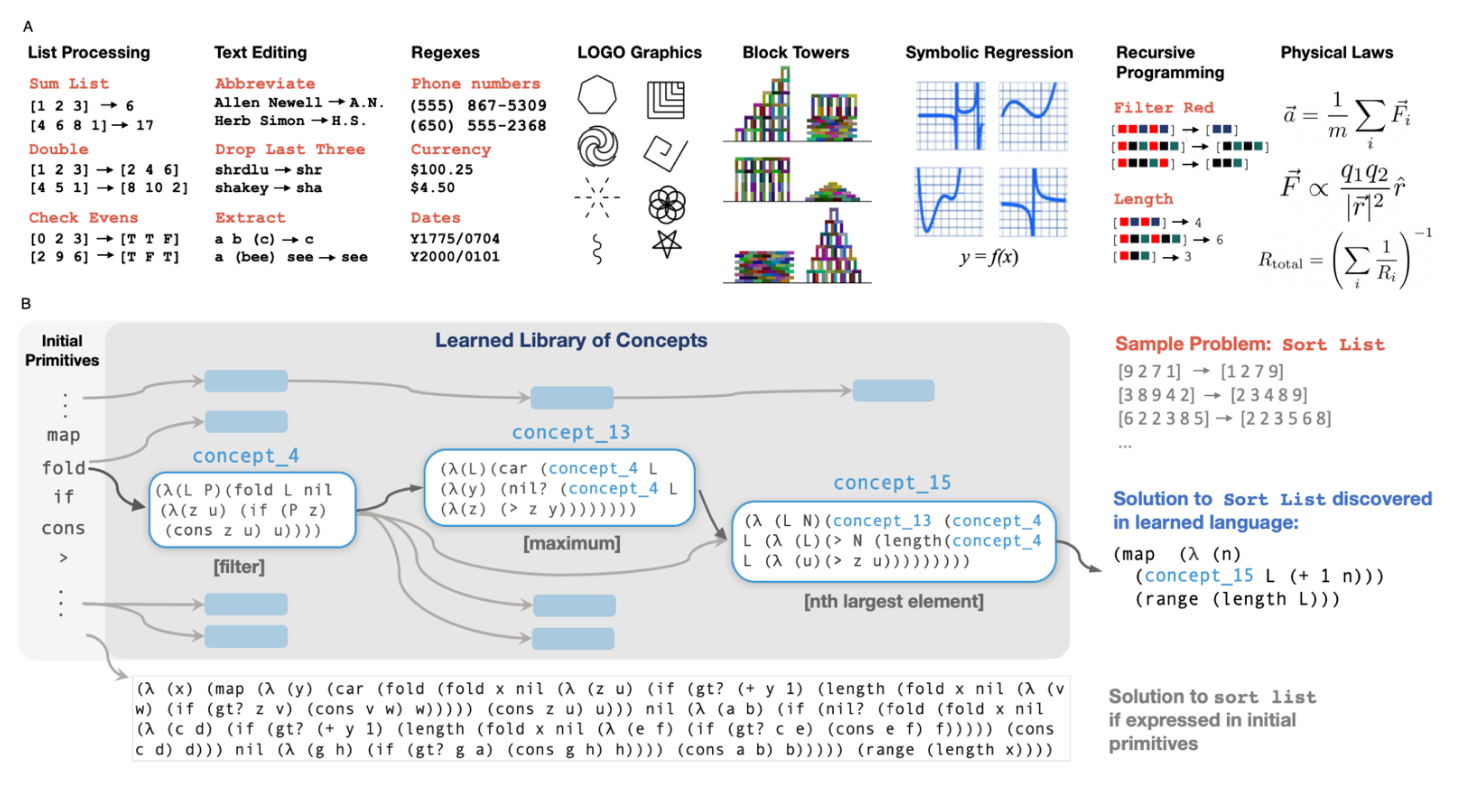
\includegraphics[width=\textwidth]{img/conc_library.png}
\label{fig:conc_library}
\caption{(A) 8 different domains of tasks. (B) Representation of the learned library of concepts. On the left we see the initial primitives from which the concepts in the middle region are composed. On the right we see a task as input-output relations and the found solution. On the bottom is the same solution expressed only with initial primitives. Image taken with permission from the original paper \cite{ellis_dreamcoder_2021}.}
\end{figure*}

The model operates in three distinct phases. 

\paragraph{Wake} In the wake phase, the objective is to find the best program $\rho$  for each task $x \in X$ DreamCoder is presented with. Each task consist of one or a few (up to $\sim10$) examples. The system synthesises the programs using a neural network as the recognition model $Q$ to search through its library $D$.

\paragraph{Sleep: Abstraction} A key component of the success of DreamCoder is the refactoring of programs. In this phase, DreamCoder consolidates new abstractions from the programs it has found during the wake phase. Experiences are replayed, and commonalities between programs are found so that they can be abstracted into new concepts to use in the future. The objective is to find programs of minimum description length (MDL). 

\paragraph{Sleep: Dreaming} The objective during the dreaming phase is to train the recognition model $Q$ to perform MAP inference by both fantasies, and replays. When fantasising, programs are drawn from the learned library as a generative model. The model is then trained on the produced tasks. This ensures a large and varied data-set to learn from and encourages out-of-distribution generalisation. Replays, simply training on previously seen task-program pairs, ensures that the model improves its predictions on the actual tasks it needs to learn, by using its programs.

A Bayesian View
- What exactly happens?
- Include the parameterization of the generative model as a bigram transition matrix (three dimensional. Parent, arg index, depth?)


\section{DeepSynth}
- Introducing different search strategies.
The two main approaches are enumerative search and sampling.
However, either way, they are first predicting weights for the PCFG and then searching or sampling from the PCFG. 
\section{Search space}
\section{Program space}
- How can we calculate the size of that space?
- Hierarchical structure 
- Abstract Syntax Trees


Recent advancements in program synthesis have seen the rise of novel techniques aimed at generating code that not only satisfies a given specification but also matches human-written code patterns. One of the most notable methods in this sphere is DreamCoder. This model, along with several other state-of-the-art (SOTA) methodologies, has shown exceptional proficiency in understanding and generating complex code structures based on given specifications.

However, a critical examination of such methods, including DreamCoder, reveals a foundational limitation: their heavy reliance on syntactical constraints. While these constraints are undoubtedly vital for ensuring the correctness of generated programs, they do not necessarily guarantee a deep understanding or utilization of semantic relationships within the code. This is akin to learning the grammar of a language but missing out on the nuances and contexts that give meaning to words and phrases.

One could argue that the attention mechanism, as seen in transformers, provides a potential solution to this limitation. The attention mechanism inherently captures dependencies between various parts of an input, no matter how distant they might be. In the context of program synthesis, such a mechanism could be instrumental in deriving and maintaining meaningful semantic relationships between different code segments. The beauty of attention is that it provides a dynamic way to weigh different parts of the input based on context, potentially allowing a transformer-based model to capture intricate semantic details of a program.

Nevertheless, a transformer's capabilities come with its own set of challenges. While the attention mechanism offers a promising avenue for capturing semantic nuances, transformers, especially when trained from scratch, require colossal amounts of data to achieve satisfactory performance. The fundamental architecture of transformers necessitates this data-driven learning, often demanding diverse and extensive training datasets that might not always be available or feasible, especially in niche areas of program synthesis. Moreover, when the goal is to create a model of human cognitive abilities, it is obvious that humans do not have access to vast amounts of data, instead, we are able to infer causal relationships, from only a limited number of examples. E.g. consider the problem \texttt{[1,2,3] $\rightarrow$ [3,2,1]}. An astute reader might promptly conclude that the list has been reversed. 
Dougs analogies 

This is where GFlowNets (GFNs) carve their niche. Contrary to the data-hungry nature of transformers, GFNs do not necessitate gargantuan datasets for efficient training. Instead, they leverage a more intuitive approach: defining a reward distribution that's directly proportional to the objects (or programs) we intend to generate. This not only streamlines the learning process but also ensures that the synthesized programs are aligned with our desired outcomes.

In the realm of program synthesis, our objectives are clearly defined. We aim to construct objects, or more specifically, pieces of code that precisely meet the given specification. This isn't just about producing syntactically correct code; it's about generating semantically rich and efficient programs that can effectively solve the specified problem without superfluous or redundant components.























\section{GFlowNet}
The problem can be formalized as finding a latent hierarchical structure from a limited set of specifications.

We can specify our GFlowNet in the realm of program synthesis as building a directed acyclic graph over abstract syntax trees.
We formalise it. 
The gfn is conditioned on the task, and so we have a conditional reward distribution $R(z|x)$, as well as a conditional forward policy $P_F(s|x)$ and partition function $Z(x)$.

I am building on the DeepSynth framework where the goal is to find programs in a domain specific language. 

The task is list editing, i.e. i get some inputs and outputs relationship and the network has to find a program that solves it. 

we want diversity, so perhaps even multiple programs that solve it. 



\section{Theory}


The trained GFlowNet gives us a the stochastic policy $\pi(a|s)$, where $a$ is an action from the action space $A$ and $s$ is a state from the state space $S$.

- Relation to Reinforcement learning
- Relation to MCMC sampling
- Relation to Variational inference. 

Since their initial publication [SOURCE], many extended and modified variants have been published. See e.g. [SOURCE, awesome GFlowNets for an overview.]




\subsection{Introduction}
A Generative Flow Network, or GFlowNet, operates as a generative model driven by a trained stochastic policy. It constructs objects $z \in Z$, where $Z$ is the space of completed states, sequentially, with each sampling probability being proportional to a reward function $R(z)$, where $R(z)$ is non-negative and integrable. GFlowNets excel in sampling diverse solutions, eliciting a high reward \cite{bengio_flow_2021}.

The state space can be visualized as a directed acyclic graph (DAG), where vertices correspond to states and edges denote transitions.

A trajectory $\tau$ is a series of state transitions commencing from an initial state $s_0$ and culminating at a terminal state, $s_n \in Z$.

The forward policy, denoted as $P_F(s'|s)$, encompasses the children of all non-terminal states in $S \setminus Z$. It inherently generates a distribution over complete trajectories:
\[ P(\tau) = \prod_{i=1}^{n} P_F(s_i|s_{i-1}) \]


Using sequential sampling from $P_F$, one can deduce a distribution $P^{\top}_F$ over terminal states:
\[ P^{\top}_F(z) = \sum_{\tau \text{ leading to } z} P_F(\tau) \]

For any reward function $R: Z \rightarrow \mathbb{R}_{\geq 0}$, GFlowNets aims to determine a parametric policy where object sampling likelihood is proportional to its reward.

The main theorem describes that if the flow function $F$ is trained such that it matches the flow-matching constraint, i.e. for any state the flow going into the state matches the flow going out of it, and the flow at terminated states $x$ is defined by the reward function $R(x)$, GFlowNet will sample terminated states with probability $\frac{R(x)}{\sum_{x\prime} R(x\prime)}$.


Since its original publication many extended and modified variants have been published.


\begin{enumerate}
    \item \textbf{TB Objective}: Trajectory Balance (TB) approach, as elaborated by Malkin et al. (2022), necessitates simultaneous learning of a forward policy, a backward policy $P_B(s|s'; \theta)$, and a scalar $Z_\theta$. The TB objective is:
    \[ L_{TB}(\tau;\theta) = \frac{Z_\theta \prod_{i=1}^{n} P_F(s_i|s_{i-1};\theta)}{\log R(z) \prod_{i=1}^{n} P_B(s_{i-1}|s_i;\theta)} \]
    
    \item \textbf{Training Dynamics}: Nullifying $L_{TB}$ ensures proportional sampling to object reward. The loss can be minimized using gradient descent with on-policy and off-policy strategies, reminiscent of reinforcement learning techniques.
    
    % \item \textbf{Subtrajectory Balance}: The SubTB methodology by Madan et al. (2023) extends the TB approach, catering to partial trajectories.
\end{enumerate}













\section{Methods}







In a probabilistic programming representation of world models and thoughts, as a type of Language of Thought, which aligns with constructivism we can conceive of the problem statement as 


In a language of thought, regardless of most details, we tend to think in a paradigm in which thoughts are compositional. In one way or another, thoughts are hierarchical.
Both in ontologies, i.e. the way concepts are structured, (animal - bird - fink) but also in the sequential nature of thought construction (as in natural language, reasoning tasks, etc.). We are creating parse trees, or abstract syntax trees. 

In a probabilistic programming paradigm, we view this as compositional functions, with the many properties of functional programming analogous to currying, etc. 

What is a thought?
[Thoughts as trajectories]

We can formalise this as a hierarchical latent structure Z.

Framing the problem.

Combinatorial search problem. 

- If we are using encoder + decoder, are we violating the Markovian Flow assumption?
    Look at the smiley example. If the NN would get [[left brow], [left brow, right brow], [left brow, right brow, smile]] as input, i.e. the sequence of the states, it would violate the assumption. but it only gets the current state, e.g. [left brow, right brow], and from that it has to infer the next step. 
    When using a decoder, we would indeed give it the whole trajectory of states, so it would violate the assumption.
    But even now i am encoding the sequence and giving the whole trajectory as input. and since the CFG is essentially a tree, there is only one parent for each state. 

It would probably be faster to do it bottom up like in HEAP search from Nathanael and from GFN-EM, then we could also use sub-trajectory balance, i.e. calculate intermediate Rewards. 

Another thing we could do is predict a bunch of terminals at once, and then combine in each step. 

Other ideas: wave function collapse

% \section{assumptions}
% \section{limitations}
% \section{biological plausibility}


- Reasons for using a GFlowNet
- Transformer allows for semantic relationships (although we still don't use control or data flow, but we could in principle)
- We want to approximate a multimodal distribution, unlike DreamCoder in which the MAP estimate refrains from finding semantically equal but syntactically different solutions. 
